\chapter{La magia dei due specchi} \label{cap:magia-specchi}

\section{La ricorsione}

A molti sarà capitato di meravigliarsi osservando la fuga delle immagini generata da due specchi contrapposti. Lo specchio numero 1 sa fare una cosa sola: riprodurre la scena che ha di fronte. Anche lo specchio numero 2 sa fare solo la stessa cosa, ma così facendo riproduce anche lo specchio numero 1, compreso la scena in esso contenuta, la quale a sua volta riproduce la scena nello specchio numero 2 e così via, all'infinito. È un fenomeno che colpisce perchè consente di sbirciare nell'infinito, normalmente inaccessibile all'esperienza umana. Questa è la ricorsione.

È molto facile creare uno schema ricorsivo attraverso il software:

\vskip 1cm

\begin{table}[H]
\begin{minipage}{1.0\textwidth}
\begin{itemize}[itemsep=-3pt,parsep=2pt]
\item[] \hspace{0.5cm}  1\hspace{8pt}TO RICORSIONE 
\item[] \hspace{0.5cm}  2\hspace{8pt}\hspace{8pt}RICORSIONE
\item[] \hspace{0.5cm}	3\hspace{8pt}END
\item[] \hspace{0.5cm}  4\hspace{8pt}
\item[] \hspace{0.5cm}  5\hspace{8pt}RICORSIONE   
\end{itemize}          	          
\end{minipage}
\end{table}

\vskip 1cm

In questo frammento di codice la Tartaruga esegue un solo comando: RICORSIONE. Non esistendo tale comando nel lessico di Logo è stato necessario definirlo con un procedura, di sapore altrettanto minimalista, perché tutto ciò che la Tartaruga deve impararare è il comando RICORSIONE stesso. Succede come negli specchi: la Tartaruga quando incontra l'istruzione TO RICORSIONE si predispone ad apprendere diligentemente il suo contenuto, che però consiste solo nel memorizzare l'istruzione RICORSIONE medesima. La Tartaruga è in grado di memorizzare sequenze di comandi che possono essere anche molto complesse, tuttavia non pensa. Una volta preso atto del contenuto della procedura, quando le viene chiesto di eseguire il comando RICORSIONE, si getta senz'altro nell'esecuzione dei comandi, inconsapevole di essere caduta in una trappola mortale! Infatti non avrà più alcun modo di uscire da questa perversa magia. Caro lettore prova a seguire la Tartaruga per vedere cosa succede, ti lascio la scoperta e la conseguente riflessione...

Se tutto ciò potrà incantare i più immaginifici, susciterà invece perplessità nei più pragmatici: a cosa può servire una cosa simile? Perchè intrappolare inutilmente la povera Tartaruga? 

Se avete fatto l'esperimento precedente, avrete visto appararire quasi subito questo messaggio: "Programma terminato: profondità ricorsiva massima (1000) superata". Evidentemente c'è chi veglia sulla sorte della Tartaruga, almeno entro certi limiti. Per esempio, l'inteprete di LibreLogo controlla quello che succede e se viene superato il limite di 1000 chiamate ricorsive ferma tutto, assumendo che ci sia qualcosa che non va. Può stupire che tutto avvenga in così breve tempo ma questo si spiega con il fatto che la Tartaruga non deve fare niente ad ogni chiamata della procedura RICORSIONE, se non richiamare un'altra volta la medesima. Poiché per fare questo tipo di operazioni il computer richiede tempi piccolissimi, frazioni di millisecondi, tutto il processo ci appare quasi instantaneo. Proviamo a rendere un po' più interessante il processo:

\vskip 1cm

\begin{table}[H]
\begin{minipage}{1.0\textwidth}
\begin{itemize}[itemsep=-3pt,parsep=2pt]
\item[] \hspace{0.5cm}  1\hspace{8pt}TO RICORSIONE R 
\item[] \hspace{0.5cm}  2\hspace{8pt}\hspace{8pt}CIRCLE R
\item[] \hspace{0.5cm}  3\hspace{8pt}\hspace{8pt}RICORSIONE R+1
\item[] \hspace{0.5cm}	4\hspace{8pt}END
\item[] \hspace{0.5cm}  5\hspace{8pt}
\item[] \hspace{0.5cm}  6\hspace{8pt}RICORSIONE 1
\end{itemize}          	          
\end{minipage}
\end{table}
\vskip 1cm

Qui abbiamo dotato la procedura RICORSIONE di un argomento, R, abbiamo aggiunto una sola istruzione, CIRCLE R, e abbiamo cambiato la chiamata ricorsiva così: RICORSIONE R+1. Quindi alla tartaruga viene chiesto di iniziare con RICORSIONE 1. A te lettore il piacere di scoprire cosa succede. Come ti lasciamo scoprire cosa succede con queste altre due varianti:

\vskip 1cm

\begin{table}[H]
\begin{minipage}{1.0\textwidth}
\begin{itemize}[itemsep=-3pt,parsep=2pt]
\item[] \hspace{0.5cm}  1\hspace{8pt}TO RICORSIONE R C
\item[] \hspace{0.5cm}  2\hspace{8pt}\hspace{8pt}IF R+ C $>$ 70 [ C = -1 ]
\item[] \hspace{0.5cm}  3\hspace{8pt}\hspace{8pt}IF R + C $<$ 50 [ C = 1 ]
\item[] \hspace{0.5cm}	4\hspace{8pt}\hspace{8pt}CIRCLE R + C
\item[] \hspace{0.5cm}  5\hspace{8pt}\hspace{8pt}RICORSIONE R+C C
\item[] \hspace{0.5cm}  6\hspace{8pt}END
\item[] \hspace{0.5cm}  7\hspace{8pt} 
\item[] \hspace{0.5cm}  8\hspace{8pt}RICORSIONE 50 1             
\end{itemize}          	          
\end{minipage}           
\end{table}
                
\vskip 1cm

\begin{table}[H]
\begin{minipage}{1.0\textwidth}
\begin{itemize}[itemsep=-3pt,parsep=2pt]
\item[] \hspace{0.5cm}  1\hspace{8pt}TO RICORSIONE N
\item[] \hspace{0.5cm}  2\hspace{8pt}\hspace{8pt}LABEL N
\item[] \hspace{0.5cm}  3\hspace{8pt}\hspace{8pt}PENUP FORWARD 10 PENDOWN
\item[] \hspace{0.5cm}	4\hspace{8pt}\hspace{8pt}IF N $>$ 20 [ STOP ]
\item[] \hspace{0.5cm}  5\hspace{8pt}\hspace{8pt}RICORSIONE N+1
\item[] \hspace{0.5cm}  6\hspace{8pt}END
\item[] \hspace{0.5cm}  7\hspace{8pt}
\item[] \hspace{0.5cm}  8\hspace{8pt}RICORSIONE 1                
\end{itemize}          	          
\end{minipage}
\end{table}

\vskip 1cm

Non sarà sfuggita l'affinità fra il concetto di ripetizione che abbiamo già visto e quello di ricorsione. Effettivamente, gli esempi che abbiamo visto possono essere riprodotti anche con l'istruzione REPEAT - il lettore può farlo per esercizio. A sua volta, l'effetto di un ciclo di ripetizione può essere ottenuto anche con la ricorsione, ponendo le operazioni da eseguire in una procedura e inserendo la chiamata ricorsiva, ovvero alla procedura stessa, come ultima istruzione. Ma chi ci vieta di effettuare la chiamata ricorsiva in altre parti della procedura, o di farne addirittura più di una? È proprio qui che la faccenda si fa interessante.

\section{Verso i frattali}

Vediamo questo esempio:

\vskip 1cm

\begin{minipage}{0.5\textwidth}
\begin{figure}[H]
   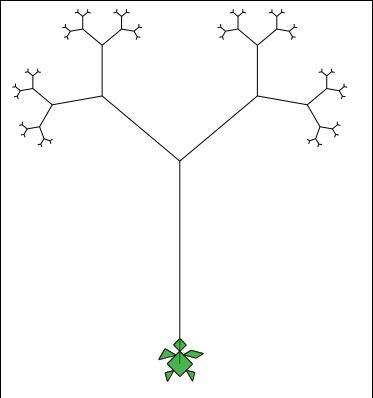
\includegraphics[width=4.0cm,trim=4 4 8 4,clip]{./images/magia-specchi/tree.png}
   \label{tree-1}
\end{figure}
\end{minipage} \hfill
\begin{minipage}{0.6\textwidth}
\begin{itemize}[itemsep=-3pt,parsep=2pt]
\item[] \hspace{0.5cm}  1\hspace{8pt}TO ALBERO LL           
\item[] \hspace{0.5cm}  2\hspace{8pt}\hspace{8pt}IF LL $<$ 2 [ STOP ]
\item[] \hspace{0.5cm}  3\hspace{8pt}\hspace{8pt}FORWARD LL LEFT 50
\item[] \hspace{0.5cm}  4\hspace{8pt}\hspace{8pt}ALBERO LL/2
\item[] \hspace{0.5cm}  5\hspace{8pt}\hspace{8pt}RIGHT 100 
\item[] \hspace{0.5cm}  6\hspace{8pt}\hspace{8pt}ALBERO LL/2
\item[] \hspace{0.5cm}  7\hspace{8pt}\hspace{8pt}LEFT 50 BACK LL
\item[] \hspace{0.5cm}  8\hspace{8pt}END
\item[] \hspace{0.5cm}  9\hspace{8pt}
\item[] \hspace{0.3cm} 10\hspace{8pt}CLEARSCREEN
\item[] \hspace{0.3cm} 11\hspace{8pt}HOME
\item[] \hspace{0.3cm} 12\hspace{8pt}ALBERO 200            
\end{itemize}
\end{minipage}                       

\vskip 1cm

La procedura ALBERO è ricorsiva perché chiama se stessa, anzi, lo fa due volte, nelle istruzioni 4 e 6, ed esegue altre operazioni successivamente alle chiamate ricorsive.

In sostanza, la Tartaruga, dopo avere pulito lo schermo (CLEARSCREEN) ed essere andata a casa (HOME) esegue una sola istruzione: ALBERO 200. Andiamo a vedere cosa succede in ALBERO. Innanzitutto ci rendiamo conto che alla variabile LL viene attribuito il valore 200. Poi, come prima cosa, la Tartaruga controlla che LL non sia inferiore a 2 e, qualora si verifichi questa condizione si interrompe l'esecuzione del programma. Ma LL è maggiore di 2 quindi si va avanti tracciando un segmento lungo 200 e girando a sinistra di 50 gradi. A quel punto ecco la prima chiamata ricorsiva a ALBERO ma con un valore dell'argomento pari a LL/2, quindi a 100. Non entriamo, per ora, "dentro" a questa chiamata e assumiamo che la Tartaruga abbia fatto quello che ci doveva fare. A questo punto la "vediamo" girare a destra di 100 gradi e poi richiamare un'altra volta ALBERO con lo stesso argomento LL/2, ossia 100. Anche qui, lasciamola "lavorare dentro" per poi vedere, che fatto questo, la Tartaruga gira nuovamente a sinistra di 50 gradi e torna indietro di LL, ovvero 200 punti. Questa descrizione è corretta ma non abbraccia tutto il processo, perché non si dice nulla su quello che succede nelle chiamate ricorsive a ALBERO. Nulla ci vieta di "entrare" anche a noi ma con un certo disagio perché non è difficile intuire che ci toccherà ripetere più volte questa operazione di "entrare" nelle chiamate ricorsive. 

In effetti la strategia di seguire passo passo l'algoritmo non funziona tanto bene quando è in gioco la ricorsione, oppure diciamo che non basta. Occorre aggiungere un'altra prospettiva a quella sequenziale. Per chiarire questo passaggio può essere utile immaginare che quando è in atto una procedura ricorsiva non c'è una sola Tarturga al lavoro ma un'intera squadra, organizzata con una precisa gerarchia.   

\begin{minipage}{0.5\textwidth}
\begin{figure}[H]
   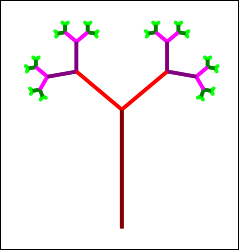
\includegraphics[width=4.0cm,trim=4 4 8 4,clip]{./images/magia-specchi/albero-fiorito.png}
   \label{tree-2}
\end{figure}
\end{minipage} \hfill
\begin{minipage}{0.4\textwidth}
In testa abbiamo la nostra solita Tartaruga, che però non disegna nulla, riducendosi all'esecuzione di ALBERO 200. Qui quello che succede è che la Tartaruga affida il lavoro alla Tartaruga Assistente Marrone, spiegandole che deve eseguire la procedura ALBERO a partire dal valore LL=200. Di altro la Tartaruga non vuole sapere e si mette pazientemente in attesa. 
\end{minipage}   

\vskip 0.5cm                    

La Tartaruga Marrone invece si mette subito all'opera, eseguendo i passi richiesti dalla procedura ALBERO esattamente come li abbiamo visti prima. Quindi disegna diligentemente il tronco lungo 200 punti, si gira a sinistra di 50 gradi ma quando arriva all'istruzione 4, si comporta nella stessa maniera, affidando il lavoro alla Tartaruga Assistente Rossa (istruzione 4), dicendole di eseguire la procedura ALBERO, nella direzione che le indica, tuttavia partendo da un valore pari a LL/2=100; dato questo ordine la Tartaruga Marrone si mette a riposo. La Tartaruga Rossa ripete lo stesso comportamento e supponiamo che abbia fatto tutto quello che doveva fare. A questo punto il controllo viene ripreso dalla Tartaruga Marrone ma non per fare molto, perché una volta giratasi a destra di 100 gradi (istruzione 5) riaffida lo stesso compito di prima alla Tartaruga Rossa (istruzione 6). Quando questa ha terminato la Tartura Marrone riparte nuovamente per girarsi di 50 gradi a sinistra e tornare indietro di 200 punti (istruzione 7), ritrovandosi così alla base del tronco.  

Emerge in questo modo il concetto di livelli di ricorsione, che noi possiamo visualizzare come i livelli delle tartarughe colorate: al primo livello opera la Tartaruga Marrone, al secondo la Tartaruga Rossa, al terzo la Tartaruga Viola e così via. Ognuna di queste non vuole sapere niente di ciò che ha fatto prima la tartaruga che le ha affidato il lavoro né di ciò che faranno quelle a cui affideranno i compiti a loro volta. Ognuna riceve delle istruzioni precise e le esegue, se deve appaltare parti di lavoro ad altre tartarughe lo fa mettendosi in attesa. 

La cosa importante è rendersi conto che con i livelli aumenta la complessità del lavoro, che si sminuzza in una successione di compiti eguali nella successione di comandi ma con parametri che vanno via via diversificandosi passando da un livello all'altro. In questo caso cambia il parametro LL che viene dimezzato ogni volta. Poiché il processo di moltiplicazione dei compiti cresce molto rapidamente con l'aumentare dei livelli non ha molto senso andare a ripercorrere pedissequamente la successione delle operazioni. Ci si "fida" che avvengano le stesse cose ad ogni livello se pur con mutate propozioni. 

Siamo qui in prossimità di due idee potenti, per dirla con Papert. La prima evoca l'importante procedimento di dimostrazione matematica per induzione, che si usa per dimostrare un'affermazione per tutti gli elementi di un insieme ordinato. Questa consiste prima nel dimostrare la verità dell'affermazione per il primo elemento dell'insieme, poi nel dimostrare che data per vera l'affermazione per l'elemento generico $n$ allora questa sia vera anche per l'elemento $n+1$. Anche qui, in qualche maniera ci si "fida" che il passaggio continui a valere per tutti gli $n$.

L'altra idea è quella di "autosimiglianza" che sta alla base del concetto di frattale. la natura frattale è posseduta da tutte quelle formazioni che non cambiano sostanzialmente aspetto osservandole a scale  anche molto diverse: nuvole, coste, cavolfiori, vasi capillari ecc. L'albero che abbiamo visto è un frattale. È sorprendente la varietà e complessità dei frattali che si possono generare anche con la nostra semplice Tartaruga. In futuro dedicheremo un capitolo a questo argomento. Per ora vediamo una variazione del nostro albero, che era effettivamente un po' troppo geometrico:

\vskip 1cm

\begin{minipage}{0.2\textwidth}
\begin{figure}[H]
   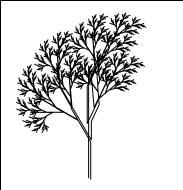
\includegraphics[width=4.0cm,trim=4 4 8 4,clip]{./images/magia-specchi/albero-meglio.png}
   \label{tree-3}
\end{figure}
\end{minipage} \hfill
\begin{minipage}{0.8\textwidth}
\begin{itemize}[itemsep=-3pt,parsep=2pt]
\item[] \hspace{0.5cm}  1\hspace{8pt}TO ALBERO LL           
\item[] \hspace{0.5cm}  2\hspace{8pt}\hspace{8pt}IF LL $<$ 5 [ FORWARD LL BACK LL STOP ]
\item[] \hspace{0.5cm}  3\hspace{8pt}\hspace{8pt}FORWARD LL/3.0
\item[] \hspace{0.5cm}  4\hspace{8pt}\hspace{8pt}LEFT 30 TREE LL*2.0/3.0 RIGHT 30
\item[] \hspace{0.5cm}  5\hspace{8pt}\hspace{8pt}FORWARD LL/6.0
\item[] \hspace{0.5cm}  6\hspace{8pt}\hspace{8pt}RIGHT 25 TREE LL/2.0 LEFT 25
\item[] \hspace{0.5cm}  7\hspace{8pt}\hspace{8pt}FORWARD LL/3.0
\item[] \hspace{0.5cm}  8\hspace{8pt}\hspace{8pt}RIGHT 25 TREE LL/2.0 LEFT 25
\item[] \hspace{0.5cm}  9\hspace{8pt}\hspace{8pt}FORWARD LL/6.0
\item[] \hspace{0.3cm} 10\hspace{8pt}\hspace{8pt}BACK LL                               
\item[] \hspace{0.3cm} 11\hspace{8pt}END
\item[] \hspace{0.3cm} 12\hspace{8pt}
\item[] \hspace{0.3cm} 13\hspace{8pt}CLEARSCREEN
\item[] \hspace{0.3cm} 14\hspace{8pt}HOME
\item[] \hspace{0.3cm} 15\hspace{8pt}ALBERO 200 
\end{itemize}
\end{minipage}                       

\vskip 1cm

